\documentclass[11pt]{article}
\usepackage[a4paper,margin=1in]{geometry}
\usepackage{graphicx}
\graphicspath{{rfigs/}}
\usepackage{enumitem}
\usepackage{xcolor}
\usepackage{mdframed}
% Toggle this to enable/disable highlights
\setlength{\parindent}{0pt}  % No indentation
\setlength{\parskip}{10pt}   % Space between paragraphs
\newif\ifhighlight
\highlighttrue % Uncomment to enable highlighting
% \highlightfalse % Uncomment to disable highlighting
\newcommand{\hl}[1]{\ifhighlight\textcolor{blue}{#1}\else#1\fi}

\newmdenv[
  topline=false,
  bottomline=false,
  skipabove=\topsep,
  skipbelow=\topsep
]{siderules}

\newcommand{\blue}[1]{\textcolor{blue}{#1}}
\newcommand{\red}[1]{\textcolor{red}{#1}}
\newcommand{\violet}[1]{\textcolor{violet}{#1}}
\newcommand{\teal}[1]{\textcolor{teal}{#1}}

\begin{document}

\section*{Response to Reviewer 1}

\begin{siderules}
\textit{Liu et al. report an analysis of a common but so far not very systematically studied phenomenon, namely the formation of a ‘dimple’ upon bringing a solid surface in contact with a thin film of a wetting fluid. The basic principle is that wetting forces suck liquid into a growing capillary meniscus very quickly, while the hydraulic resistance of the thin liquid film limits the supply of fluid. This results in the transient formation of a ‘dimple’ of reduced film thickness surrounding the solid object, which is a slice of beet in the present work. Eventually the dimple relaxes under the influence of capillary forces. The work provides a clear description of the experiments; the phenomenon is nicely documented and reproduced in numerical solutions of the lubrication equation. The ms. certainly deserves publication. I have few minor comments that the authors may want to consider. }
\end{siderules}

\begin{siderules}
\textbf{Comment 1:} \textit{I was not aware of the Reynolds ridge that the authors describe in the introduction, which involves Marangoni effects. While interesting, I agree with the authors that this effect is probably irrelevant for the present phenomenon. More interesting, however, is the effect of the transient ‘dimple’ or ‘ripple’ formation upon spreading of drops of pre-existing liquid films (or upon depositing a solid sphere onto such a film). This branch of literature would establish another – arguably more relevant – link to pre-existing art. See e.g. Garcia-Gonzales et al. Soft Matter 2023 and Jalaal et al. JFM 2019, which provide a good bibliography of the ‘ripple’ phenomenon going back all the way to Tanner’s paper from 1979 who also discussed spreading on pre-existing liquid films and reported the formation of a dimple, which was shown to reach a minimum thickness of 0.82 times the initial thickness.}
\end{siderules}

\textbf{Response:} We thank the reviewer for bringing the literature on ``ripple spreading'' to our attention. The two papers present interesting ripple dynamics around a solid sphere / a spreading viscoelastic droplet. The findings highlight the importance of dynamics on capillary adhesion. The ripple phenomenon resembles the key observation of this work, and the analysis on the evolution of length scales is relevant to this work. Hence, we include the following sentence in the introduction to link our work to the visco-capillary ripple literature:

\hl{
``The formation and the evolution of the dimple resembles the ripple spreading in relaxing thin polymer films (Cormier 2012, McGraw 2012, Jalaal 2019) and upon the contact between a solid and a thin liquid film (Garcia-Gonzalez 2023).''
}

\bigskip
\begin{siderules}
\textbf{Comment 2:} \textit{P.11: the authors argue that the scaling exponent $\alpha$ is reminiscent of Tanner’s large exponents for the spreading of a drop on a flat surface. This argument feels a bit fortuitous: the exponent in Tanner’s law arises from the divergence of the friction at the contact line in combination with mass conservation. Here, the minimum thickness at the dimple, which controls the relaxation process is several tens of micrometers. On the other hand, the authors argue that the spreading takes place on the vertical part of the surface. Do they mean side of the beet slice? Isn’t the effective friction there taken into account via eq. 5? If the interest is in the spreading on the side wall, shouldn’t one then analyze the maximum height vs. time? Please elaborate in the ms. on the connection to Tanner's law.}
\end{siderules}

\textbf{Response:} We thank the reviewer for pointing out the issue with our tentative argument. The velocity of the contact line, as the reviewer pointed out, is already prescribed in Eq.5. When the contact angle approaches the stationary contact angle, the velocity of the contact line goes to zero due to the divergent friction.

There are two sources of friction/drag in this phenomenon: the contact line and the dimple. To see which one dominates, we look at the temporal evolution of the contact line on the side wall. In Fig.~\ref{fig:contact-line}, we plot both experimental and simulation data for contact line height over time. Interestingly, we observe that it takes a longer time for the contact line of the thinner film to reach a ``stationary'' height. This observation suggests that, for sufficiently small $h_0$ (around 0.2 mm), the viscous dissipation at the dimple is the dominant friction/drag. 

\begin{figure}
    \centering
    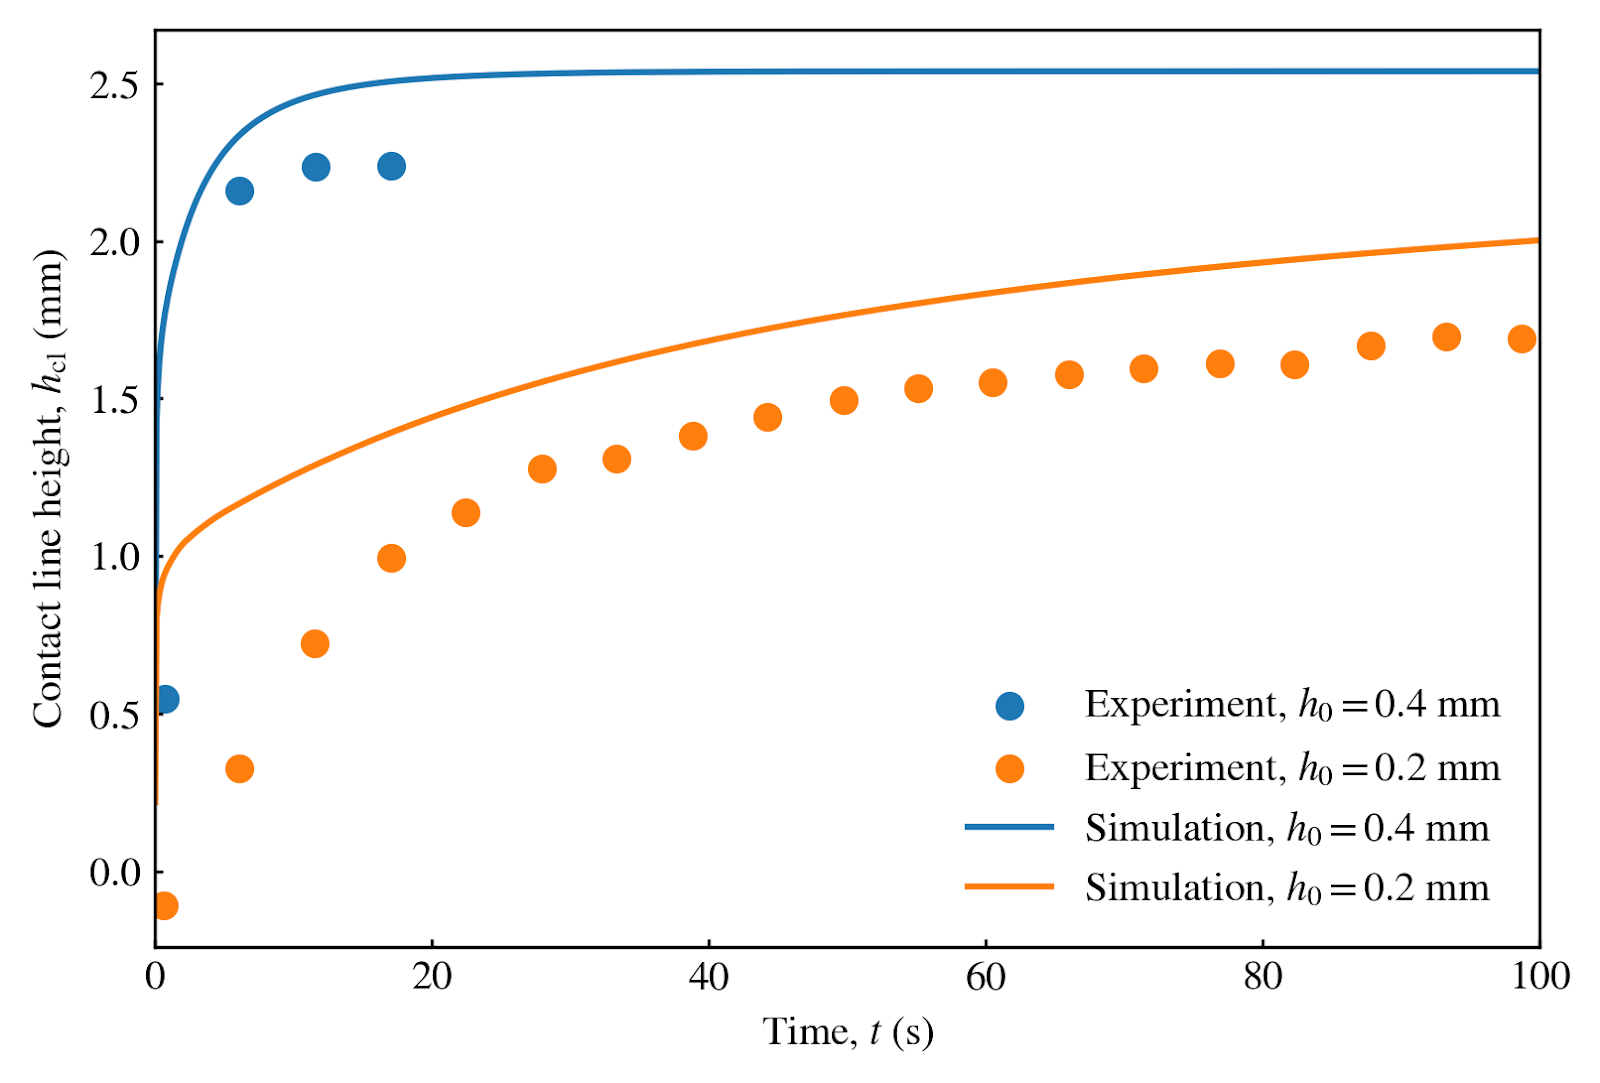
\includegraphics[width=0.6\linewidth]{contact_line_motion._thicknesspng.png}
    \caption{Experimental and simulated temporal evolution of contact line.}
    \label{fig:contact-line}
\end{figure}

\hl{
Therefore, using Tanner’s law to understand the scaling of dimple time is not justified. 
We removed the discussion on Tanner’s law, and added a section to show our revised understanding of the scaling exponent. 
See Section~III~E in the revised manuscript for detailed discussion.
}

\bigskip
\begin{siderules}
\textbf{Comment 3:} \textit{Fig. 4: labels of the last two panels should be d) and e).}
\end{siderules}

\textbf{Response:} We thank the reviewer for pointing out the typo. We fixed it. 

\bigskip
\begin{siderules}
\textbf{Comment 4:} \textit{P. 9: the characteristic time scale that arises from the lubrication equation is $t_\mathrm{lub}=3 \mu L/ \sigma  (L/h_0)^3$. Why does this time scale not matter here and is replaced by eq. 2 instead? Please elaborate.}
\end{siderules}

\textbf{Response:} We appreciate the insightful comment on the time scale analysis. 
The lubrication equation scales
\begin{eqnarray}
        \frac{\partial h}{\partial t} &=& \frac{1}{3\mu} \frac{\partial}{\partial x} \left( h^3 \frac{\partial p}{\partial x} \right) \\
        \frac{\partial h}{\partial t} &=& \frac{1}{3\mu} \frac{\partial}{\partial x} \left( h^3 \frac{\partial }{\partial x} \left( \sigma \frac{\partial^2 h}{\partial x^{2}} + \frac{\rho g h}{2} \right) \right) \\   
        Ca \frac{\partial h^*}{\partial t^*} &=& \frac{1}{3} \left(\frac{\mathcal{H}}{\mathcal{L}}\right)^4 \frac{\partial}{\partial x^*} \left( h^{*3} \frac{\partial }{\partial x^*} \left( \frac{\partial^2 h^*}{\partial x^{*2}} + Bo \, {h^*} \right) \right) \, ,        
\end{eqnarray}
where $H$ and $L$ are the characteristic height and length and $Ca = \mu V/\sigma$ and $Bo = \rho g \mathcal{L}^2 /\sigma$. Assuming $\mathcal{L}$ is the length of the initial film, our experiments have $\mathcal{L} \sim 20$ mm, which is larger than the capillary length. Then, the Bond number becomes $\mathcal{O} (10)$. 

As the reviewer mentioned, when the Bond nummber is small, the lubrication time scale becomes  
\begin{equation}
    \mathcal{T} \sim \frac{\mu}{\sigma} \frac{\mathcal{L}^4}{\mathcal{H}^3} \,.
\end{equation}

However, when the Bond number is large (most experiments), the lubrication time scale can be expressed as 
\begin{equation}
    \mathcal{T} \sim \frac{\mu}{\rho g} \frac{\mathcal{L}^2}{\mathcal{H}^3} \,.
\end{equation}

In current experimental conditions, we can assume that the lubrication time scale is proportional to the length square. Also, this is supported by the simulation results shown in the figure below.

\begin{figure}[ht]
    \centering
    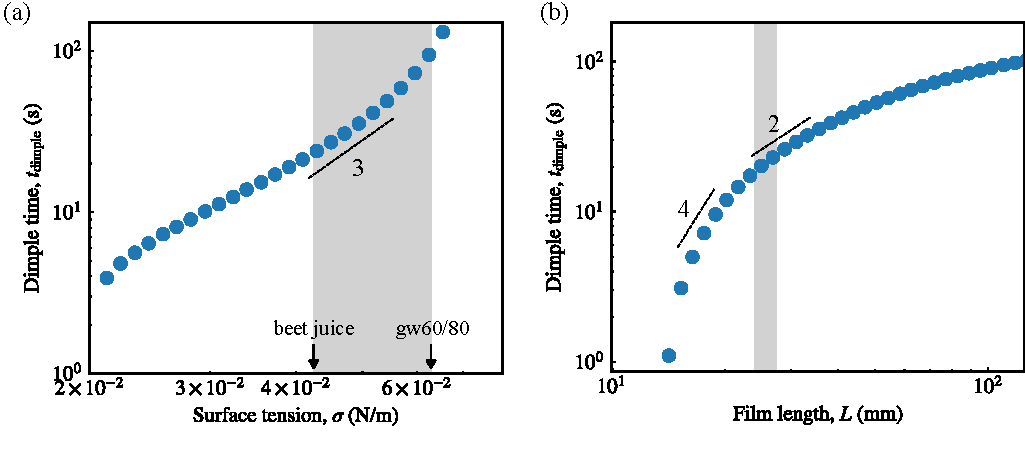
\includegraphics[width=0.9\linewidth]{Figures/surface_tension_and_film_length.pdf}
    \caption{Dimple time vs. film length. Within our experimental range of $L \sim 24$ mm, the dimple time is proportional to the square of the film initial length.}
    \label{fig:tention_length}
\end{figure}


\hl{
In the revised manuscript, we wrote details in Section III-E about the dimple time scale and further scaling arguments. 
}



% Short answer: approximating the pressure at dimple using the film length $L$ is off, i.e.
% %
% $$
% \sigma\frac{h_0}{L^2} \ll P_\mathrm{dimple}.
% $$
% %
% This is because the dimple is not fully relaxed and the curvature is still localized to a length shorter than the film length $L$. 
% In the original manuscript, we chose $h_0$ as the local length scale.
% This choice resulted in $P_\mathrm{surface}\sim \sigma / h_0$, and in turn Eq.~2 in the original manuscript.

% \begin{figure}[ht]
%     \centering
%     \includegraphics[width=.8\linewidth]{different_lengths.png}
%     \caption{Simulated surface evolutions of thin films of different length $L\in\{ 16, 24, 100\}$ mm, from the same initial thickness $h_0=0.3$ mm.
%     The locations of dimple and bulk apex are marked by blue and red dots. 
%     The insets show the evolutions of $h_\mathrm{min}$ and $h_\mathrm{max}$.
%     }
%     \label{fig:different-lengths}
% \end{figure}

% The dimple relaxation is driven by both surface tension and gravity, as can be seen in the Young-Laplace equation (Eq.~4 in the manuscript). 
% It is important to identify the dominant driving force, in order to yield the best approximation of $t_\mathrm{dimple}$.
% At $t_\mathrm{dimple}$, which force dominates depends on the length of the film $L$.
% As illustrated in Fig.~\ref{fig:different-lengths}, when $L$ is short, surface tension is dominant; when $L$ is long, gravity is dominant.
% To see the relative contributions of surface tension and gravity more quantitatively at $t_\mathrm{dimple}$, we make a phase diagram of $P_\mathrm{surface}/P_\mathrm{gravity}$ with respect to the film length $L$ and initial thickness $h_0$, as shown in Fig.~\ref{fig:gc-pd}. 
% $P_\mathrm{surface}$ and $P_\mathrm{gravity}$ are defined as the two terms in the Young-Laplace equation, namely:
% %
% \begin{equation}
%     P_\mathrm{surface} = -\sigma \left[1+\left(\frac{\partial h}{\partial x}\right)^2\right]^{-3/2} \frac{\partial^2 h}{\partial x^2}\bigg|_{x=x_\mathrm{min}},
% \end{equation}
% %
% \begin{equation}
%     P_\mathrm{gravity}= \rho g (h_\mathrm{max}-h_\mathrm{min}),
% \end{equation}
% %
% where $x_\mathrm{min}$ is the horizontal location of the dimple, $h_\mathrm{max}$ and $h_\mathrm{min}$ are the film apex height and the dimple height, respectively (all at $t_\mathrm{dimple}$).

% % Let's take a look at an example, where $h_0=0.3\;\mathrm{mm}$, $L=24\;\mathrm{mm}$.
% % At $t_\mathrm{dimple}\approx 24\;\mathrm{s}$, the curvature pressure at the dimple is $P_\mathrm{dimple}\approx 1\;\mathrm{Pa}$. The two approximations are $\sigma h_0 /L^2\approx 0.02\;\mathrm{Pa}$ and $\sigma/h_0\approx 140\;\mathrm{Pa}$.
% % Neither is a good approximation.

% \begin{figure}
%     \centering
%     \includegraphics[width=\linewidth]{Figures/phase_diagram}
%     \caption{
%     \textbf{Phase diagrams and two $t_\mathrm{dimple}$ approximations.}
%     (a) Pressure contribution $\ln P_\mathrm{gravity}/P_\mathrm{curvature}$ phase diagram.
%     (b) Film thickness approximation $\ln h_\mathrm{max}/h_0$ phase diagram.
%     (c) Compare $t_\mathrm{dimple}$ approximations by Eq.~\ref{eq:approx1} and Eq.~\ref{eq:approx2} with experimental and simulation data. 
%     }
%     \label{fig:phase-diagram}
% \end{figure}

% Our experiments, as indicated by the dashed box in Fig.~\ref{fig:phase-diagram}, $L\approx24$ mm.
% According to the phase diagram, gravity is more important at $t_\mathrm{dimple}$ at this $L$.
% Thus, it is more appropriate to use the balance between gravity and viscous drag to estimate $t_\mathrm{dimple}$:
% %
% \begin{equation}
%     \rho g h_0 \sim \frac{\mu U L}{h_0^2},
% \end{equation}
% %
% which gives a time scale $\tau_g$
% %
% \begin{equation}\label{eq:approx1}
%     \tau_g \sim \frac{\mu L^2}{\rho gh_0^3}.
% \end{equation}
% %

% Figure~\ref{fig:phase-diagram}(c) shows a comparison between simulated $t_\mathrm{dimple}$ and the gravity approximation $\tau_g$ for $h_0\in [0.24, 0.4]$ mm.
% For large $h_0$, $\tau_g$ approximates $t_\mathrm{dimple}$ well. 
% For small $h_0$, however, the deviation becomes pronounced.
% In this limit, $h_0$ is no longer a good approximation of the characteristic height of the thin film.
% Instead, the film apex, $h_\mathrm{max}$, is a better approximation (see Fig.~\ref{fig:phase-diagram}(b) for a comparison between $h_\mathrm{max}$ and $h_0$ for various film geometries).
% So, a better approximation of $t_\mathrm{dimple}$ is
% %
% \begin{equation}\label{eq:approx2}
%     t_\mathrm{dimple} \sim \frac{\mu L^2}{\rho gh_\mathrm{max}^3}.
% \end{equation}
% %
% Figure~\ref{fig:phase-diagram}(c) also shows the $h_\mathrm{max}$ approximation, which obviously agrees with experimental and simulated data better. 

% \hl{
% In the revised manuscript, we replaced the scaling argument based on the balance between surface tension and viscous drag.
% We added Section~III~E to discuss the new understanding of the time scale, with a particular focus on the film geometry effect. 
% }

\bigskip
\begin{siderules}
\textbf{Comment 5:} \textit{Fig.~5 and description on p.~10: the time scales are unclear: clearly, the first profile cannot be the moment when the beet is brought in touch with the film because the film must have been flat initially. What determines $t=0$? This seems arbitrary.}
\end{siderules}

\textbf{Response:} The reviewer is correct that $t=0$ was not clearly defined. We define the time of the initial contact between the beet and the liquid film as $t=0$. The first scanned profile corresponds to the scan between $t=0$ and $t=1$ as each scan takes about 1 second (see the schematic in Fig.~\ref{fig:first-scan}). In the manuscript (Figs.~4 and 5), we used the averaged time over the duration of each scan. For example, the first scanned data are noted as $t=0.5$ s, the midpoint of the scan interval. 

\begin{figure}[ht]
    \centering
    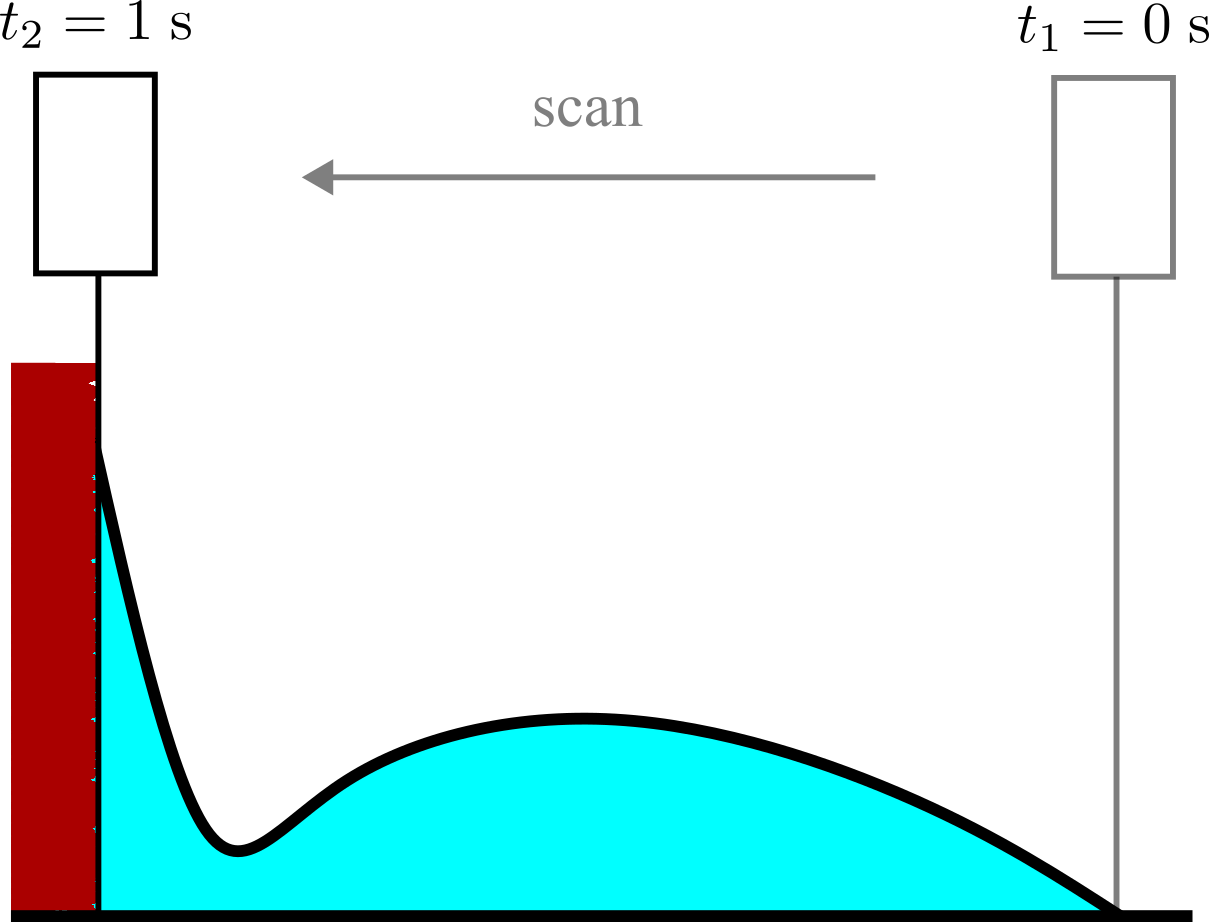
\includegraphics[width=0.4\linewidth]{illustrate_scan_time.png}
    \caption{Surface scan illustration.}
    \label{fig:first-scan}
\end{figure}

\bigskip
\begin{siderules}
\textbf{Comment 6:} \textit{Same topic: the text on p.~10 says that ``different color codes for time are used to differentiate simulation data from experimental data.'' I see identical color codes and times in Figs.~5a and 5b. Please elaborate on the different color scales and mention explicitly whether there are any fit parameters or not to make the absolute time scales match.}
\end{siderules}

\textbf{Response:} We thank the reviewer for catching this error. The color codes for time in Figs. 5a and 5b are exactly the same.
No fit parameter is included to match the time scales. We originally used two different color codes for experiment and simulation (Fig.~\ref{fig:different-color}). 
However, we noticed that readers might wish to compare the two surface profiles at each time, so we changed the figure to use the same colormap for both experiment and simulation. The writing of “different color codes” was out-dated. We change the sentence to \hl{``The same color code for time is used to allow comparison of the surface evolutions.''}

\begin{figure}[ht]
    \centering
    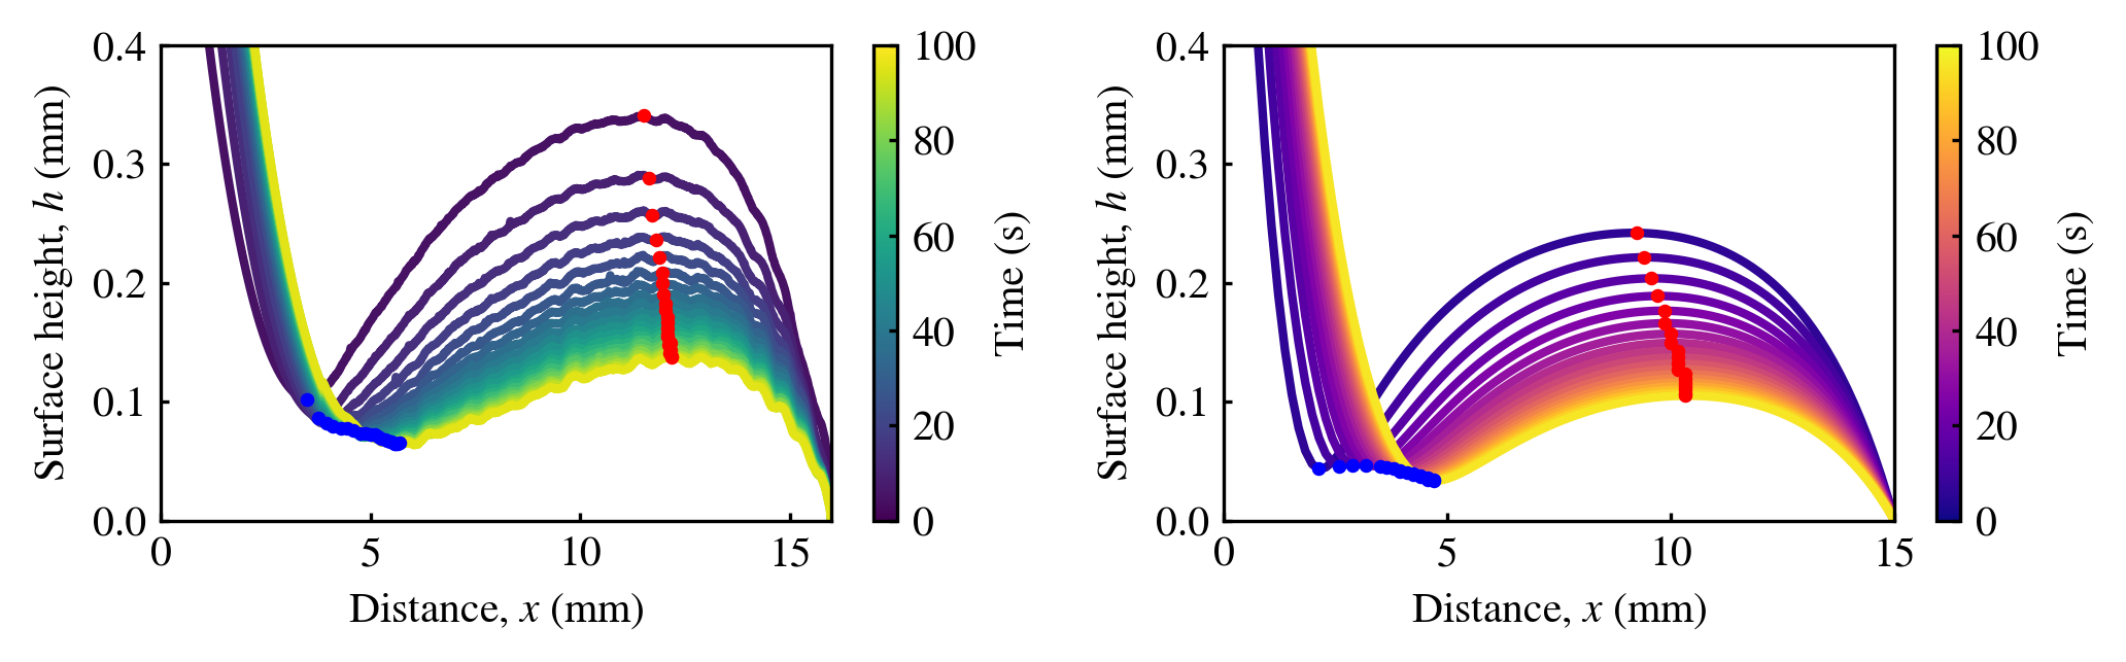
\includegraphics[width=0.9\linewidth]{different_color_codes.png}
    \caption{The original Figs.~5a and 5b with different color codes.}
    \label{fig:different-color}
\end{figure}

\bigskip
\begin{siderules}
\textbf{Comment 7:} \textit{Discussion: the authors argue that the dimple caused by the rise of the capillary meniscus rather than suction of the beet. I believe this; probably the beet is pretty saturated with fluid to begin with. But does this matter? If the authors would deposit a dry porous disc onto their film, shouldn’t this quickly suck fluid from the film and induce dimple formation as well?}
\end{siderules}

\textbf{Response:} The reviewer is absolutely correct about this. If a dry beet is placed in a thin liquid film, the suction would be even stronger and what we would likely observe the disjoining of the liquid film. 
Actually, in our simulation version 1, we modelled the beet slice as a porous disc.
Based on the pore size ($\sim 50\;\mathrm{\mu m}$), we estimated the negative pressure that arises from the pores to be around 1000~Pa. 
This simulation failed to converge, because the suction flow was too drastic.

After screening a range of negative pressure values, we realized that by lowering the boundary negative pressure to the order of 10 Pa, we could get thin film behaviors very similar to the experiment. 
This way, we realized that the main driving force of the dimple / fringe formation was the capillary rise on the side wall of the beet. 

As the reviewer suggested, the porousness of the beet does matter. In terms of absorbing capacity, the pores can probably host even more fluid, if it is dried beforehand. However, if we consider porousness the only source of suction, we would be curious why a very saturated slice of beet can still induce a fringe. Our manuscript answers this question by showing the alternative suction mechanism: \emph{wall capillary rise}.

We believe that readers will likely have similar concerns on this point. So, we add the following paragraph to the ``Conclusion and discussion'' section of the manuscript. 

\hl{
While our work identifies the wetting of the sidewall as the primary source of suction, one may wonder whether the beet porousness can also play a role. 
First, we note that in an experiment, the beet slices we used were pretty saturated with juice, so we did not expect the pore suction to be significant. 
We also tried to model the suction flow by considering the negative pressure caused by the pores, which drives the suction flow. The negative pressure was on the order of 1000 Pa ($\approx \sigma /r$ where $r $ is a typical pore radius; $\sim 50 \,\mu\mathrm{m}$ \cite{beetpore}). 
When running the numerical simulation with this negative pressure as the boundary condition, the solver failed because the suction was so drastic that no convergence could be reached. 
After screening a range of negative pressure values, we realized that by lowering the boundary negative pressure to the order of 10 Pa, we could get thin film behaviors very similar to the experiment. 
This way, we realize that the main driving force of the dimple/fringe formation is the capillary rising on the side wall of the beet, which indeed induces negative pressure on the order of 10 Pa. 
}

\bigskip
\begin{siderules}
\textbf{Comment 8:} \textit{Marangoni effect and profile asymmetry: I agree that this can be arbitrarily complicated for actual beet juice. But in the experiments with the glycerol-water mixtures, why would there be a substantial Marangoni effect? Does the asymmetry depend on the system? this would be easy to test, e.g. by adding surfactant intentionally to see whether this affects the asymmetry.}
\end{siderules}

\textbf{Response:} We speculate that the asymmetry of the surface profiles comes from the Marangoni effect. Since we use pickled beet in our experiment, the ``juice'' likely contains vinegar and other acidic compounds, which evaporate faster at the far end contact line and cause surface tension gradient, which can induce Marangoni flow away from the beet. Although we did not test this explicitly, we observed more symmetric surface profiles in glycerol-water mixtures, as suggested by the reviewer. See the Fig.~\ref{fig:beet-and-gw} for a comparison between beet surface and 60\% glycerol-water surface. 

\begin{figure}
    \centering
    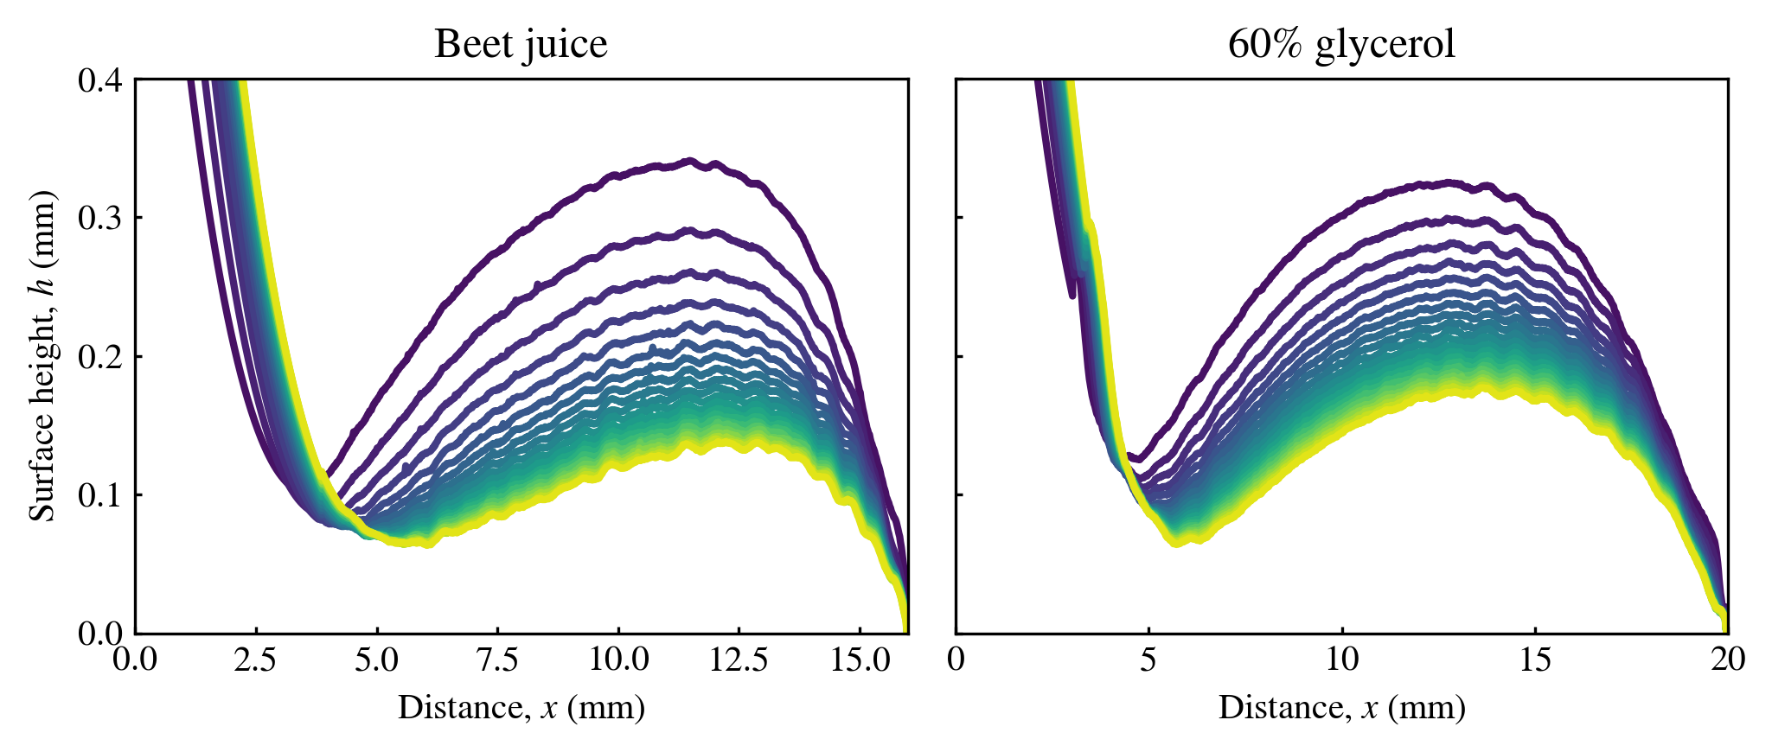
\includegraphics[width=0.8\linewidth]{beet_and_gw.png}
    \caption{Surface profiles of beet juice (left) and 60\% glycerol-water (right) over time. }
    \label{fig:beet-and-gw}
\end{figure}


\end{document}
